\documentclass{article}
\usepackage{amsmath}
\usepackage{bm}
\usepackage{tikz}
\usetikzlibrary{arrows.meta}

\begin{document}

\begin{figure}[h]
    \centering
    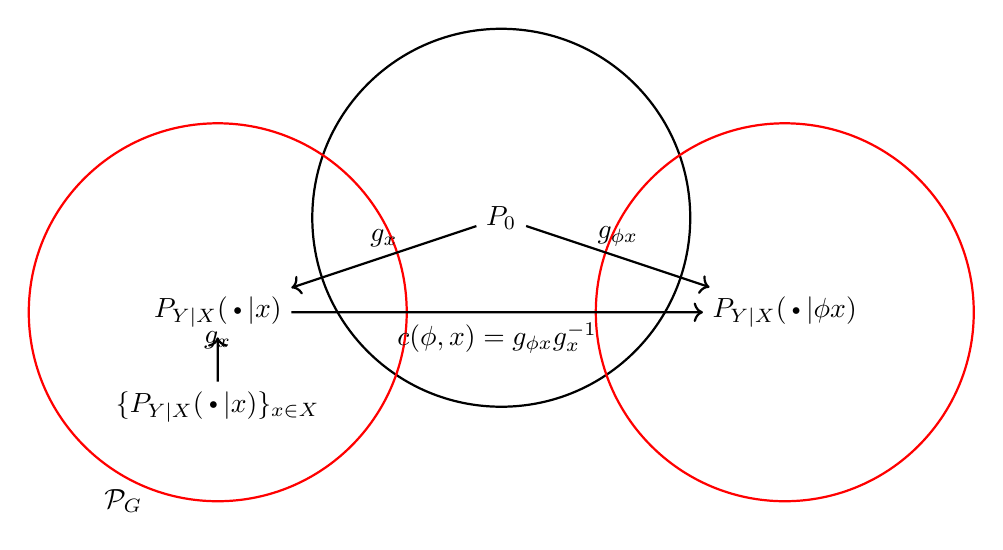
\begin{tikzpicture}[scale=1.2]
        % Define the nodes
        \node (P0) at (0, 0) {$P_0$};
        \node (PX) at (-3, -1) {$P_{Y|X}({\,\vcenter{\hbox{\tiny$\bullet$}}\,} |x)$};
        \node (PYX) at (3, -1) {$P_{Y|X}({\,\vcenter{\hbox{\tiny$\bullet$}}\,} |\phi x)$};
        \node (GX) at (-3, -2) {$\{P_{Y|X}({\,\vcenter{\hbox{\tiny$\bullet$}}\,} |x)\}_{x \in \mathbb{X}}$};
        
        % Draw the circles
        \draw[thick] (P0) circle (2);
        \draw[red, thick] (PX) circle (2);
        \draw[red, thick] (PYX) circle (2);
        
        % Draw the arrows
        \draw[->, thick] (P0) -- node[above] {$g_{\phi x}$} (PYX);
        \draw[->, thick] (P0) -- node[above] {$g_x$} (PX);
        \draw[->, thick] (PX) -- node[below] {$c(\phi, x) = g_{\phi x}g_x^{-1}$} (PYX);
        \draw[->, thick] (GX) -- node[above] {$g_x$} (PX);
        
        % Label the group
        \node at (-4, -3) {$\mathcal{P}_{\mathbb{G}}$};
    \end{tikzpicture}
    \caption{Suppose the set of distributions $\{P_{Y|X}({\,\vcenter{\hbox{\tiny$\bullet$}}\,} |x): x \in \mathbb{X}\}$ lies in a transformation model $\mathcal{P}_{\mathbb{G}} = \{g_*P_0 : g \in \mathbb{G}\} \subseteq \mathcal{P}(\mathbb{Y})$. For each $x \in \mathbb{X}$ there is an element $g_{x}$ of the group $\mathbb{G}$ such that $P_{Y|X}({\,\vcenter{\hbox{\tiny$\bullet$}}\,} |\phi x) = g_{x*}P_0$. If we transform $x$ with $\phi$, there is also an element $g_{\phi x}$ such that $P_{Y|X}({\,\vcenter{\hbox{\tiny$\bullet$}}\,}|x) = g_{\phi x*}P_0$. This allows us to move directly from $P_{Y|X}({\,\vcenter{\hbox{\tiny$\bullet$}}\,}|x)$ to $P_{Y|X}({\,\vcenter{\hbox{\tiny$\bullet$}}\,}|\phi x)$ using the coboundary $c(\phi,x): (\phi,x) \mapsto g_{\phi x}g_x^{-1} \in \mathbb{G}$. Note that this coboundary does not depend on $P_0$ and so is shared by (infinitely) many other conditional distributions. By directly modelling the coboundary instead of $P_{Y|X}$, we can therefore improve robustness to model mis-specification.}
    \label{fig:coboundary}
\end{figure}

\end{document}